% THIS IS SIGPROC-SP.TEX - VERSION 3.1
% WORKS WITH V3.2SP OF ACM_PROC_ARTICLE-SP.CLS
% APRIL 2009
%
% It is an example file showing how to use the 'acm_proc_article-sp.cls' V3.2SP
% LaTeX2e document class file for Conference Proceedings submissions.
% ----------------------------------------------------------------------------------------------------------------
% This .tex file (and associated .cls V3.2SP) *DOES NOT* produce:
%       1) The Permission Statement
%       2) The Conference (location) Info information
%       3) The Copyright Line with ACM data
%       4) Page numbering
% ---------------------------------------------------------------------------------------------------------------
% It is an example which *does* use the .bib file (from which the .bbl file
% is produced).
% REMEMBER HOWEVER: After having produced the .bbl file,
% and prior to final submission,
% you need to 'insert'  your .bbl file into your source .tex file so as to provide
% ONE 'self-contained' source file.
%
% Questions regarding SIGS should be sent to
% Adrienne Griscti ---> griscti@acm.org
%
% Questions/suggestions regarding the guidelines, .tex and .cls files, etc. to
% Gerald Murray ---> murray@hq.acm.org
%
% For tracking purposes - this is V3.1SP - APRIL 2009

\documentclass{acm_proc_article-sp}
\usepackage{caption}
\usepackage{graphicx}
\usepackage{float} 
\usepackage{multirow}
\usepackage{cite}
\usepackage{url}
\begin{document}

\title{What Makes A Digital Steward:}
\subtitle{A Competency Profile Based On The National Digital Stewardship Residencies}

\author{
  \begin{tabular}{c}
    % 1st. author
    Karl-Rainer Blumenthal\\
       \affaddr{Internet Archive}\\
       \email{karlb@archive.org}
  \end{tabular}%
  \begin{tabular}{c}
    % 2nd. author
    Peggy Griesinger\\
       \affaddr{George Mason University}\\
       \email{mgriesin@gmu.edu}
  \end{tabular} \\[10pt]\\
  \begin{tabular}{c}
    % 3rd. author
    Julia Kim\\
       \affaddr{Library of Congress}\\
       \email{juliakim@loc.gov}
  \end{tabular}
  \begin{tabular}{c}
    % 4th. author
    Shira Peltzman\\
       \affaddr{University of California, Los Angeles}\\
       \email{speltzman@library.ucla.edu}
  \end{tabular}
  \begin{tabular}{c}
    % 5th. author
    Vicky Steeves\\
       \affaddr{New York University}\\
       \email{vicky.steeves@nyu.edu}
  \end{tabular}
}

\date{25 April 2016}

\maketitle

\begin{abstract}
Digital stewardship is the active and long-term management of digital objects towards their preservation for and unencumbered access by future generations. Although the field is rapidly maturing, it still lacks a comprehensive competency profile for practitioners. This is due in part to the relative youth of the field, and to the fact that being an effective steward of digital materials requires highly specialized training that is best acquired through hands-on work. Given the key role that competency profiles play in the design of curricula and job postings, the lack of one hinders the training and education of professionals for these positions. This paper provides a profile of the skills, responsibilities, and knowledge areas that define competency in digital stewardship, based on a close study of the projects undertaken in the National Digital Stewardship Residency program (NDSR). The authors use a triangulated research methodology in order to define the scope of the profile, qualitatively analyze the competencies articulated among NDSR project descriptions, and quantitatively evaluate those competencies' importance to professional success.  The profile that results from this research has implications for current and future digital stewards: training designed with this profile as its basis will focus on the skills most needed to be an effective digital steward, and therefore can guide both graduate and professional development curricula alike.
\end{abstract}

\keywords{digital stewardship, National Digital Stewardship Residency, NDSR, education, training, digital preservation}

\section{Introduction}
Although digital preservation is a young field, there are now more scholarship, tools, and resources that address the long-term stewardship\footnote{For the purposes of this paper, "digital stewardship" is defined as the active and long-term management of digital objects towards their robust preservation for and unencumbered access by future generations, inclusive of all subfields of labor and expertise previously defined among professional surveys and studies as digital curation, data curation, data management, digital archiving, digital preservation, and digitization. Digital stewards include data librarians, digital asset managers, digital archivists, and all manner of administrators who seek to align disparate digitization and digital preservation efforts.} of digital material than ever before. In recent years there has been a notable expansion of educational and training resources in particular, including workshops, symposia, conferences, and professional development curricula. However, as the 2015 National Agenda for Digital Stewardship asserts, "[g]enuine interest and motivation to learn about a subject cannot be taught in a workshop or training session; similarly, knowledge about standards and practices in an evolving field is best gained through direct, practical experience."\cite{1} In short, being an effective steward of digital material requires more extensive and specialized training than can be acquired through traditional means.

What, then, makes a digital steward? Despite the acknowledgment that stewards must possess a particular skillset, there has not yet been sufficient scholarship performed to identify a competency profile for digital stewards, as exists in other professional communities. A competency profile succinctly articulates the specific skills, responsibilities, and knowledge areas required to practice in one's profession, and is therefore instrumental to setting training and education goals. Perhaps it is due to the field's relative youth that so many analyses of it have focused principally on the surrounding literature--most commonly surveys of graduate school curricula or job advertisements--rather than on the backgrounds and training of practitioners themselves. But as the amount of digital material entering libraries, archives, and museums worldwide continues to grow, developing successful training goals for the next generation of stewards is an increasingly vital pursuit.  

The lack of any cogent competency profile for this field is significant because competency profiles are used in the creation of job ads and curriculum development, which in turn affects how the field and its practitioners succeed in and improve their profession. In spite of this, the Agenda singles out the National Digital Stewardship Residency (NDSR hereafter) as an especially successful training model due to the fact that it allows recent graduates to gain practical, hands-on experience in the field managing digital stewardship projects. Although measuring the long-term impact of this program on the field at large would be premature\footnote{Although it is not a longitudinal analysis, the Council on Library and Information Resources (CLIR) is at the time of writing conducting a cross-cohort assessment of the entire NDSR program in order to evaluate the significance of the residency experience for the residents and their host institutions, and to identify common success factors across the various residencies.\cite{2}}, the project descriptions created by host institutions for both current and former residents yield valuable information. Both the wide variety of projects and activities covered as well as the fact that they explicitly outline goals and responsibilities for each individual resident and project makes them ideal for determining the skillset and expertise required to successfully perform the professional duties of a digital steward. 

The authors developed a competency profile for digital stewards by using a three-pronged approach: 1) reviewing literature on the topics of emerging digital stewardship roles, responsibilities, expected practices, and training needs; 2) qualitatively analyzing current and completed NDSR project descriptions, which outline project tasks and deliverables; and 3) quantitatively analyzing the results from a survey conducted of former and current residents that identified the range and types of competencies required to successfully complete each project. The result is a profile of the skills, responsibilities, and knowledge areas that define competency in digital stewardship, which will create a clearer understanding of the on-the-job skills required of digital stewardship professionals in the hopes of informing future professional and curricula development in the field.

\section{About NDSR}
NDSR was created by the Library of Congress, in partnership with the Institute of Museum and Library Services (IMLS), with the mission to "build a dedicated community of professionals who will advance our nation's capabilities in managing, preserving, and making accessible the digital record of human achievement."\cite{3} In its pilot year (2013-2014) NDSR matched ten recent graduates with mentors at ten cultural heritage institutions in order to develop, apply, and advance emerging digital stewardship practices and their own knowledge and skills in real-world settings. Since then, IMLS has granted funding to five additional NDSR programs among cultural heritage organizations throughout the country.

The program involves competitive selection processes for both host institutions and residents. Host institutions are selected on the basis of criteria such as their ability to provide higher-level support and mentorship to residents, as well as the significance of their proposed projects. These projects can be as broad in scope as institutional assessments and policy writing, or as narrow as documenting the particular application of software within a larger workflow. Applicants must be U.S. citizens or able to work in the U.S., as well as recent graduates of post-baccalaureate degrees. 

Although residents' salaries are paid through IMLS grant funds, they are regarded as regular employees by their host institutions and measures are taken to ensure that they are incorporated into the fabric of their institutions' workplaces. This is balanced by the fact that the residency is an apprenticeship program in which important criteria are learning outcomes and job placement within the field after its completion. Each NDSR program supplements on-site support with workshops and trainings designed to foster professional growth. Residents are also strongly encouraged to publicize their projects through presentations and conference participation. 

\section{Literature Review}
Competency profiles are a common way for information management professions to express educational and/or professional benchmarks. These include foundational professional concepts, information resources, research standards, lifelong learning expectations, and management principles and ethics, among other things. The American Library Association's "Core Competencies of Librarianship," for instance, establishes a baseline for those things that every "person graduating from an ALA-accredited master's program in library and information studies should know and, where appropriate, be able to employ."\cite{4} At least 16 affiliated or closely related professional organizations have adopted similar statements. \cite{5}

Studies of training needs and efficacy \cite{6, 7, 8} cite the lack of a commonly accepted profile for digital stewardship as confounding to efforts to design complementary curricula. Alternative approaches in the U.S.,\cite{9, 10}, U.K.\cite{11}, and internationally\cite{12, 13} survey professionals actively working in digital stewardship roles to identify their core competencies in order to broadly identify gaps and opportunities in the training and education of current and future professionals. Efforts continue to develop rigorous digital stewardship curricula among select ALA-accredited programs in library and information science. They range from exhaustively deductive matrices of technical proficiencies\cite{14} to inductive and fieldwork-based practicum programs.\cite{15}

Studies both external\cite{16} and internal\cite{17} to the Society of American Archivists (SAA) were instrumental to the creation of that organization's Digital Archives Specialist (DAS) Curriculum and its corresponding certification program, which at the time of writing provides the archival profession's most succinct, widely disseminated, and professionally supported profile of the "core competencies" for digital archivists. These competencies are summarized in seven statements of ability, such as: "\#1. Understand the nature of records in electronic form, including the functions of various storage media, the nature of system dependence, and the effect on integrity of records over time." \cite{18} Digital stewards outside of the archives domain would benefit from similarly rigorous research and output.

The logic for identifying competency indicators differs across the above efforts, but the authors took especial interest in the methodology chosen for the \textit{Information: Curate, Archive, Manage, Preserve} (iCAMP) curriculum development project, which reduces the language of data management job advertisements to summaries of the job titles, experience requirements, and knowledge and skill expectations that they contain\cite{19}. The results are too specific to the data management domain and generalized in their language to answer this paper's questions regarding digital stewardship writ large. However, they provide a useful precedent for the application of qualitative data analysis tools to perform comparable document analysis on a corpus of residency project descriptions that the authors believe are both more broad in their professional scope and specific in their language. 

Less rigorous, more impromptu investigations\cite{20, 21} also mine the corpus of job advertisements for language articulating the specific competencies desired by information organizations hiring digital archivists. These inquiries provide useful insight into the emerging lexicon of digital archives, but leave open to question how many of these articulated competencies and skills are the core responsibilities for their hires, and towards which future professionals must train.

The literature review reveals an opportunity to provide digital stewards with an overarching competency profile and statement that span various specializations within the field, but which also articulate requirements concretely enough to guide graduate and professional education and training goals. 

\begin{table*}[t!]
\caption{\textbf{Code categories, their frequencies and sub-codes from the document analysis.}}
\begin{tabular}{lll}
\textbf{Code category} & \textbf{Frequency} & \textbf{Sub-Codes} \\
Technical skills & 397 & Format migration/transcoding \\
\multicolumn{2}{l}{\multirow{9}{*}{}} & Metadata \\
\multicolumn{2}{l}{} & Workflow enhancement/development \\
\multicolumn{2}{l}{} & Audio/video \\
\multicolumn{2}{l}{} & Digital asset management \\
\multicolumn{2}{l}{} & Digitization \\
\multicolumn{2}{l}{} & Coding/scripting \\
\multicolumn{2}{l}{} & Implementation of hardware/software \\
\multicolumn{2}{l}{} & Web archiving \\
\multicolumn{2}{l}{} & Qualitative and data analysis skills \\
Professional output responsibilities & 275 & Metadata crosswalk/guidelines \\
\multicolumn{2}{l}{\multirow{4}{*}{}} & Report/recommendations \\
\multicolumn{2}{l}{} & Survey/inventory \\
\multicolumn{2}{l}{} & Teaching materials/toolkits \\
\multicolumn{2}{l}{} & Scholarly output \\
Communication skills & 148 & Presentation \\
\multicolumn{2}{l}{\multirow{5}{*}{}} & Written output \\
\multicolumn{2}{l}{} & Workshop/training \\
\multicolumn{2}{l}{} & Interact/liaise with internal staff/stakeholders \\
\multicolumn{2}{l}{} & Interact/liaise with external stakeholders \\
\multicolumn{2}{l}{} & Public outreach \\
Research responsibilities & 118 & Literature review \\
\multicolumn{2}{l}{\multirow{2}{*}{}} & Survey of standards/best practices \\
\multicolumn{2}{l}{} & Environmental scan \\
Project management abilities & 92 & Managing resources \\
\multicolumn{2}{l}{} & Managing people \\
Knowledge of standards and best practices & 62 & Metadata \\
\multicolumn{2}{l}{\multirow{2}{*}{}} & Data management \\
\multicolumn{2}{l}{} & Repository management \\
Personality requirements & 30 & Attention to detail \\
 &  & Flexible \\
 &  & Enthusiastic
\end{tabular}
\label{my-label}
\end{table*}

The authors used a triangulated approach to create a profile of digital stewardship competencies. The literature review provided an initial sample of commonly used summary terminology for skills, knowledge areas, and responsibilities typically applied in practice. This informed the authors' distillation of 35 NDSR project descriptions through document analysis\footnote{Document analysis is a systematic procedure for analyzing and interpreting data generated from documents; in qualitative research, document analysis is often used to corroborate findings from other data sources such as surveys, interviews, etc.\cite{22}}, the results of which provided the authors the precise terminology with which to construct a survey instrument. 

Project descriptions for both New York residency cohorts\cite{23} and the second of the two cohorts in each Boston\cite{24} and Washington, D.C.\cite{25} were retrieved from each cohort's official website. Project descriptions for the initial Boston\cite{26} and Washington, D.C.\cite{27} residency cohorts were retrieved from the archived instances of those cohorts' official websites made available through the Internet Archive's Wayback Machine.  

\section{Research Methods}
\begin{figure*}[!t]
  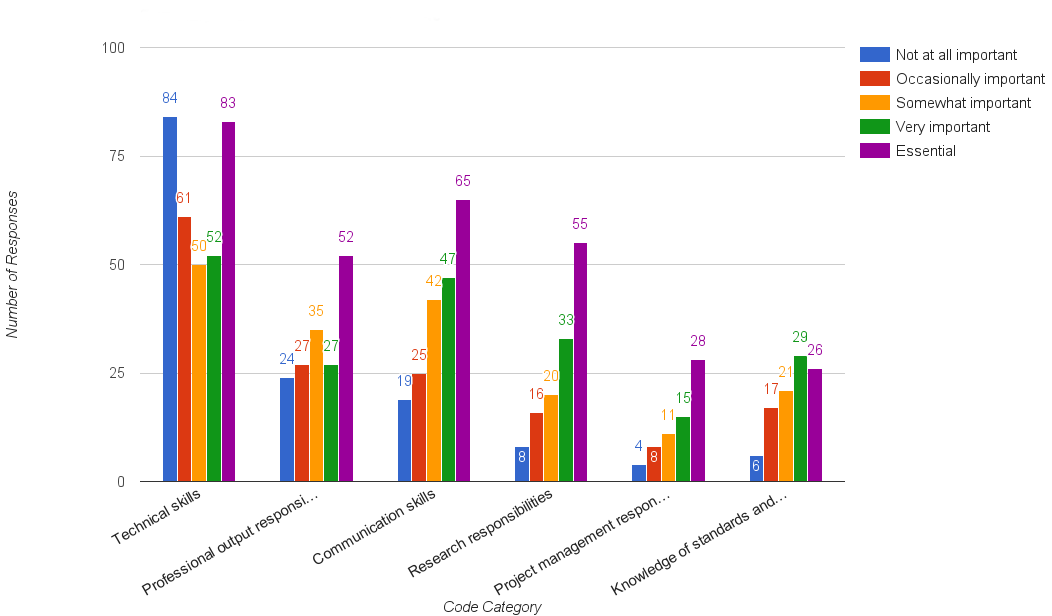
\includegraphics[scale=0.5]{total_skills.png} 
   \label{Figure 1.}   
    \caption{\textbf{Total distribution of frequency of responses over code categories.}}
\end{figure*}

The authors used a social science research methodology called grounded theory\cite{28} to analyze the qualitative data (project descriptions). Research using grounded theory begins with a collection of qualitative data that the researcher then reviews and re-reviews. During this process, the researcher tags specific quotes, words, or phrases as evidence, and assigns them "codes" that represent larger ideas.\cite{29} As data is iteratively reviewed, these codes can be grouped into concepts and ultimately categories, which become the basis for a new thesis or theory. This differs from traditional qualitative methodology because it creates its theoretical framework inductively, rather than relying upon an existing one.\cite{30}

The authors used this method to code for attributes expected of each resident. In order to do this, the authors used NVivo\footnote{Produced by QSR International: http://www.qsrinternational.com/product}, a proprietary qualitative data analysis software designed for researchers working with data that requires deep levels of analysis. NVivo was chosen because of its real-time version control, which was useful because the research team was geographically distributed. Two of the authors performed an initial blind review of the materials, using a predetermined codebook\footnote{A codebook describes and defines the codes for which the authors searched.} based on an initial sampling of the dataset and the literature review. 

Although the document analysis could provide the authors with a baseline understanding of the attributes that the residents were intended to develop, the authors also sought to examine how the projects had been borne out in practice. To accomplish this, the authors designed and implemented an online survey of current and past residents. By comparing the findings of the document analysis and the survey, the authors could assign quantitative weight to any similarities, differences, or unanticipated but necessary competencies.

The overarching code categories became the question blocks and the sub-codes became the corresponding rating matrix of individual questions within the survey instrument (see Supplementary Materials). The authors chose to exclude \textit{Personality requirements} (see Table 1) from the survey because these are general traits common to job advertisements across professions, rather than specific to digital stewardship. 

The authors used Qualtrics\footnote{Produced by Qualtrics: https://www.qualtrics.com/}, a proprietary research software used to enable online data collection through building survey instruments, because it was readily available via an institutional license, randomized question order, and anonymized participants down to the IP address.

Initially, four survey invitations were sent to the list of participants using the Qualtrics email function, or "mailer." The mailer allows for complete anonymity in the data collection: the authors could not see who had completed or not completed the survey. This also allowed the authors to send out individualized, anonymous links, to separate respondents in bulk. Nine current or former residents did not participate by the date on which the survey was originally scheduled to end. To get as close to a full dataset as possible, each author sent a follow-up email to four-to-seven participants to remind them of the deadline. The link to the survey included in these emails was still anonymous and did not record IP addresses, but was no longer unique to each recipient. 

The authors acknowledge several methodological issues with the data collection for this study. The first is that the authors are included in the dataset as participants. The most significant issue is that the authors effectively studied themselves; they designed, tested, and discussed the survey before deployment. As a result, they did not take the survey blind. Not only did this differentiate them from the rest of the participants, which could potentially skew the data, but it also introduced the potential for nonresponse bias\cite{31}. However, the authors randomized the questions to mitigate the latter issue. Although the authors recognize that participating in their own research is unorthodox, they felt that it was essential to equally represent all of the different NDSR projects, locations, and cohorts in the survey results were they to recuse themselves. Moreover, because the authors all belonged to the same 2014-15 NDSR in New York cohort, those projects would not have been represented in the survey results. The authors felt that the benefits of including their responses  outweighed the potential costs of excluding their responses from the dataset. 

Another potential problem was the fact that fifteen of the participants took the survey before they completed their residencies. This introduced a possibility for survey bias \cite{33}. They might not have been able to answer the optional questions regarding 1) post-NDSR job functions, and 2) additional skills necessary to complete their residencies. However, since the current residents could answer all the required questions (they were more than halfway through their residencies during data collection), they were still included in the participant population. 

The authors' final concern was with sending individual emails to participants. This demystified some of the initial anonymity afforded by using the Qualtrics mailer. Some participants replied to these individualized emails, indicating they had already taken the survey (some even providing the date), or that they had not taken part but would do so shortly. The authors promptly deleted these emails permanently, and no records of them remain. Given the already small sample size, the authors felt that having as close to a complete dataset as possible was so impactful to the results that the follow-ups were necessary. 

\section{Results}
This study had two main outputs: the results of the document analysis (qualitative), and the results of the survey (quantitative). Through examining both, the authors could create a matrix of the competency areas vital to the National Digital Stewardship Residencies.  

\subsection{Document Analysis}
Two of the authors coded the project descriptions. In order to compare their interpretations of the data, the authors used the NVivo "coding comparison" feature to determine that they had a 90\% agreement rate on the codes, and then met to reconcile the 10\% of cases in which their coding differed. The seven resulting high-level code categories represent the overall categories of competencies required to perform as a digital steward. These were informed by terminology from the literature review and the initial sampling of the qualitative dataset.

Seven coded categories of competence in residency-related functions emerged from the analysis: \textit{Technical skills}; \textit{Knowledge of standards and best practices}; \textit{Research responsibilities}; \textit{Communication skills}; \textit{Project management abilities}; \textit{Professional output responsibilities}; and \textit{Personality requirements}. The authors iteratively reviewed the qualitative data in order to identify sub-codes that more specifically represent the competency areas applied in the performance of the residencies. The minimum number of sub-codes per category was two, within \textit{Project management abilities}, and the maximum was ten, within \textit{Technical skills} (see Table 1). 

Due in part to their extensive range of skills, \textit{Technical skills} has the highest frequency of appearances in the data (397). The second-highest is \textit{Professional output responsibilities} (275). \textit{Personality requirements} appear the least, at 30 in total. 

\subsection{Survey Responses}
\begin{figure}[b!]
\centering
	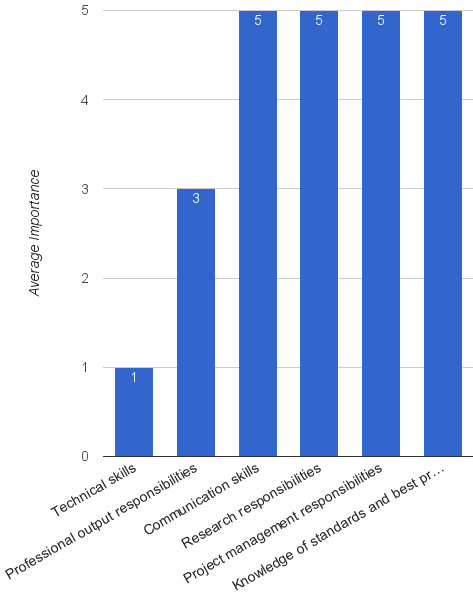
\includegraphics[keepaspectratio, scale=0.4]{modal_average.png} 
	\label{Figure 3.}
	\caption{\textbf{Modal average of code categories.}}
\end{figure}

\begin{table*}[t!]
\centering
\caption{\textbf{Responses per sub-code with descriptive statistics.}}
\resizebox{\textwidth}{!}{%
\begin{tabular}{llllllll}
 &  & \multicolumn{5}{l}{\textbf{Response Counts}} &  \\
\textbf{Code Category} & \textbf{Sub-Code} & \textbf{1} & \textbf{2} & \textbf{3} & \textbf{4} & \textbf{5} & \textbf{Mode} \\
Technical skills & Format migration/transcoding & 10 & 6 & 10 & 4 & 3 & 1,3 \\
 & Metadata creation and manipulation & 5 & 5 & 5 & 7 & 11 & 5 \\
 & Workflow enhancement/development & 1 & 1 & 3 & 7 & 21 & 5 \\
 & A/V preservation & 14 & 6 & 3 & 2 & 8 & 1 \\
 & Digital asset management & 2 & 3 & 5 & 8 & 15 & 5 \\
 & Digitization & 11 & 8 & 5 & 5 & 4 & 1 \\
 & Coding/scripting & 10 & 10 & 6 & 4 & 3 & 1,2 \\
 & Hardware/software implementation & 6 & 7 & 7 & 7 & 6 & 3 \\
 & Web archiving & 18 & 7 & 3 & 1 & 4 & 1 \\
 & Qualitative data analysis & 7 & 8 & 3 & 7 & 8 & 2,5 \\
Professional output responsibilities & Metadata documentation & 6 & 4 & 7 & 9 & 7 & 3,5 \\
 & Reports/recommendations & 0 & 3 & 0 & 2 & 28 & 5 \\
 & Surveys and/or inventories & 1 & 9 & 8 & 7 & 8 & 2 \\
 & Teaching materials/toolkits & 7 & 7 & 10 & 3 & 6 & 3 \\
 & Scholarly output (ie. annotated bibliographies, white papers, etc.) & 10 & 4 & 10 & 6 & 3 & 1,3 \\
Communication skills & Presentations (webinars, conferences, in-person stakeholder meetings, etc.) & 1 & 2 & 6 & 9 & 15 & 5 \\
 & Written output (blog posts, journal articles, etc.) & 2 & 1 & 14 & 9 & 7 & 3 \\
 & Workshops and trainings & 3 & 8 & 9 & 7 & 6 & 3 \\
 & Internal Interactions & 0 & 0 & 1 & 8 & 24 & 5 \\
 & External Interactions & 4 & 5 & 6 & 8 & 10 & 5 \\
 & Public Outreach (social media, public events, etc.) & 9 & 9 & 6 & 6 & 3 & 1,2 \\
Research responsibilities & Literature reviews & 6 & 7 & 9 & 5 & 6 & 3 \\
 & Surveys of best practices and standards & 0 & 5 & 4 & 7 & 17 & 5 \\
 & Environmental scans (e.g. reviewing practices at peer institutions) & 1 & 3 & 2 & 11 & 16 & 5 \\
 & Needs assessment/gap analysis & 1 & 1 & 5 & 10 & 16 & 5 \\
Project management abilities & Managing project resources (ie. workflows, tools, documentation, etc.) & 2 & 2 & 2 & 9 & 18 & 5 \\
 & Managing people (ie. vendor relations, intern/staff supervision, etc.) & 2 & 6 & 9 & 6 & 10 & 5 \\
Knowledge of standards and best practices & Metadata & 1 & 5 & 5 & 14 & 8 & 4 \\
 & Data management & 4 & 5 & 7 & 8 & 9 & 5 \\
 & Repository management (TRAC, TRD, OAIS, etc.) & 1 & 7 & 9 & 7 & 9 & 3,5
\end{tabular}%
}

\label{my-label}
\end{table*}
The survey was open from March 14 to April 1, 2016. After excluding \textit{Personality requirements}, each of the six code categories had one required question, which took the form of a rating matrix (see Supplementary Materials). Each sub-code (see Table 1) represented a row of the matrix, and participants were asked to rank competencies on a five-point Likert scale from "Not at all important" (1) to "Essential" (5) (matrix columns). The survey had a 94\% response rate, having received 33 participant responses out of a total group of 35. The authors analyzed the frequency of responses in each code block in order to determine what the most impactful categories and individual competencies were to achieving residency goals.  

Respondents identified "Essential" competencies frequently throughout the code categories. In four of the six categories, more sub-codes were deemed "Essential" than they were deemed any other level of importance, and in each case by a margin of at least seven responses. \textit{Technical skills} had a higher combined frequency of responses for "Not at all important" and "Occasionally important" than it did for "Very important" and "Essential," which drove down its overall importance rating. Only three more respondents deemed \textit{Knowledge of standards and best practices} "Very important" than those who deemed it "Essential."

The category of \textit{Technical skills} had the lowest average importance of the six codes, and \textit{Professional output responsibilities} had the second-lowest. The other four codes were all deemed "Essential" on average by the participants (see Figure 3). 

\subsubsection{Technical Skills}
\begin{figure*}
\centering
	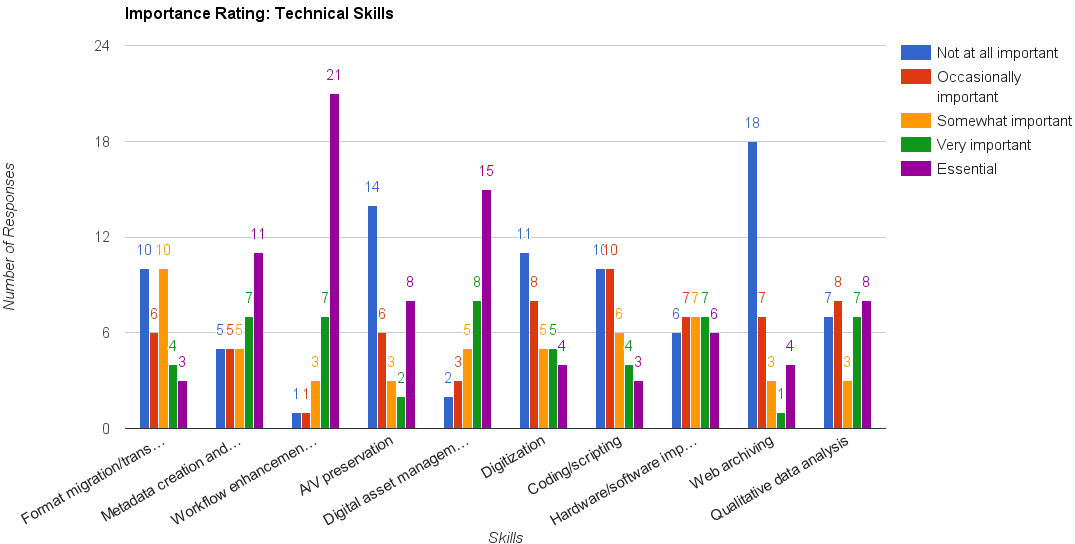
\includegraphics[keepaspectratio, scale=0.5]{tech_skills.png} 
	\label{Figure 4.}
	\caption{\textbf{Breakdown of technical skills code category.}}
\end{figure*}
Perhaps the most striking aspect of the data was the \textit{Technical skills} category. \textit{Technical skills} had the most mixed results of any category in the survey, which could be due in part to the fact that it had the highest number of granular competency areas (sub-codes). The result was a clear disparity in the distribution of responses per importance level. The outlier in \textit{Technical skills} with the lowest importance rating was \textit{Web archiving}, which lowered the overall importance found in Figure 3. \textit{Workflow enhancement} was also an outlier; it was rated as the most essential technical skill by a margin of seven responses. 

\subsection{Optional Questions}
After answering the required questions above, survey respondents were invited to answer three optional questions.

\subsubsection{Quantitative}
An optional question in the survey asked the participants whether or not their experience in NDSR was relevant to their current employment. Every participant answered this question, with 90\% (30 participants) say yes, while 10\% (3 participants) answering no.

\subsubsection{Qualitative}
The last two questions in the survey were open-ended questions that asked participants for feedback in longer-form writing. The first question asked participants to identify any competencies not addressed in the survey. 33\% (11 of 33) of respondents answered this question. The authors could not ascribe any particular pattern to these responses, however several of them further described a competency or competencies from the survey as applied to their specific project. The second question asked for any additional feedback or comments. 18\% (6 of 33) answered the second question. These answers were not analyzed using the qualitative methods above due to the low frequency and disparate topics covered, some of which again answered the previous optional question. 

\section{Conclusions}
Learning from the competency areas that were described in the NDSR projects and identified by residents as being especially important (i.e. achieving a surveyed modal average of 4 [Very important] or 5 [Essential]), a competency statement representing this profile could read as follows:

\begin{quote}
Effective digital stewards leverage their technical skills, knowledge of standards and best practices, research opportunities, communication skills, and project management abilities to ensure the long-term viability of the digital record.

In order to accomplish this, they cultivate their skill developing and enhancing new and existing digital media workflows, managing digital assets, and creating and manipulating these assets' metadata. They commit to the successful implementation of these new workflows by reliably managing both project resources and people.

They maximize the impact of their professional practice by soliciting regular input from stakeholders both internal and external to their institutional setting. They articulate and document the standards and practices that address these needs by creating policies, professional recommendations, and reports, which requires that they maintain current and and expert knowledge of standards and best practices for metadata and data management in their respective sectors.

They articulate and document the practices that address these needs by creating policies, professional recommendations, and reports, which requires that they maintain current and expert knowledge of metadata and data management standards in their respective sectors.

Digital stewards are qualified to manage, preserve, and provide access to various new and/or challenging forms of media. They may also engage in, among other things: coding and scripting; digitization; hardware and software implementation; public outreach; and special media format management and migration.
\end{quote}

The authors conclude that while there are some fundamental competencies required of digital stewards, digital stewardship also encompasses niche skills that are role-specific. Several \textit{Technical skills} were far more important to some projects than to others, and therefore could be considered specialized, rather than fundamental skills. There was a clear bimodal distribution for \textit{Technical skills} (sub-codes in this category were deemed "Not at all important" 84 times and "Essential" 85 times). The authors posit that while job postings often list \textit{Technical skills} as being essential, this study indicates that they are not always essential to all jobs in practice. 

These split distributions apply to \textit{Technical skills} sub-codes as well. For example, respondents were evenly split when gauging the importance of both \textit{Hardware/software implementation} and \textit{Qualitative data analysis}. These skills were unambiguously important to half of the respondents, but unambiguously unimportant to the other half. \textit{Web archiving} distinguishes itself in this regard as a particularly niche skill--"Essential" to four respondents, but "Not important at all" to eighteen. By contrast, \textit{Workflow enhancement} is a universally important skill, having been deemed "Essential" twenty-one times and "Not important at all" only once.   

By analyzing the project descriptions of the National Digital Stewardship Residencies, the authors enumerated the competency areas that define digital stewardship across a broad swath of applications. By surveying the residents responsible for successfully completing these residencies, they were also able to highlight fundamental competency areas that therefore belong in any profile of an effective digital steward.

\section{Implications and Future Work}
While the majority of competencies (sub-codes) surveyed for this study were definitively fundamental (had a mode $\geq$ 4) or specialized (had a mode of $\leq$ 2), there were thirteen that could not be as conclusively categorized. Of these, there were five that had a mode of 3, meaning the majority of the participants labeled these as "Somewhat important." These are: \textit{Hardware/software implementation}, \textit{Written output}, \textit{Workshops and trainings}, \textit{Teaching materials/toolkits}, and \textit{Literature review}. Seven sub-codes had multiple modes, showing disagreement among the participants as to the relevance of the skill for successfully completing their digital stewardship work. These are: \textit{Format migration/transcoding}, \textit{Coding/scripting}, \textit{Qualitative data analysis}, \textit{Public outreach}, \textit{Repository management}, \textit{Metadata documentation}, and \textit{Scholarly output}. The authors refrained from assigning these sub-codes into either the "Fundamental" or the "Specialized" tiers. The authors included them in this study's resulting competency statement as examples of further and increasingly specialized areas of work for which digital stewards are qualified, however, determining the place that these specific thirteen sub-codes hold in the overall profile of competencies for digital stewards presents an opportunity for future research.

It is important to note that this study's qualitative analysis was based on descriptions of projects, all of which were inherently time-limited and some of which were deliberately narrow in focus. While it was beyond the scope of this study, the diversity of project types among NDSR cohorts may also have affected the results. The specificity of certain projects, coupled with the fact that they were all designed to be accomplished in a relatively short time-frame, may have impacted our results to some degree--perhaps enough so to merit a new study that is based on a different set of data. However, the 90\% affirmation among this study's survey respondents implies that these competencies extend to digital stewardship positions beyond NDSR. The authors encourage using a similarly triangulated methodology to analyze competency areas found among permanent position descriptions and their incumbents. In particular, a follow-up study of those who have completed National Digital Stewardship Residencies and are now in permanent digital stewardship positions could do so while counterbalancing any possible bias of this study towards competencies that apply disproportionately to short-term appointments. 

Finally, it is worth noting the fact that all residencies took place in the U.S.A., and consequently that this research is not international in scope. This presents an important area for future research, which might involve conducting a comparable study built on job descriptions culled from a variety of national contexts. Contrasting the results of such a study with the competency profile presented here would perhaps enable the construction of a stronger and more well-rounded profile overall.

This research has implications for current and future digital stewards alike: The resulting profile can be used to guide graduate and professional development curricula, and training designed with this profile as its basis will focus on the skills most needed to be an effective digital steward. For instance, this study suggests that although specific technical skills are viewed as highly important in different settings, a much larger majority of projects required skills less bound to a particular technology or media, like documentation creation and workflow analysis. The high level of agreement regarding the importance of writing reports and communicating internally also bolsters a need for digital stewards to not only possess a deep understanding of their field, but to effectively disseminate their work to others. This new profile illustrates the fundamental competencies that must be cultivated by digital stewards in order to succeed in the profession. 

\section{Supplementary Materials}
The authors welcome and encourage others to extend and reproduce their study, and have made all research materials, including the survey instrument and data, freely available at the following URL: \url{https://osf.io/xfc26}

\bibliographystyle{unsrt} 
\bibliography{2016-10-03_iPRES_NDSRLongPaperBiblio}

%\balancecolumns 

\end{document}